% The generic preamble
\documentclass[10pt,letterpaper,fleqn,titlepage]{article}

% Define packages to use
\usepackage{natbib}
\usepackage[dvips]{graphicx,color}
\usepackage{amsmath,amssymb}
\usepackage{bm}
\usepackage{caption}
\usepackage{xr}
\usepackage{ifthen}
\usepackage[dvipdfm,colorlinks,linkcolor=blue,citecolor=blue,urlcolor=blue]{hyperref}
\usepackage{fancybox}
\usepackage{textcomp}
\usepackage{alltt}
%\usepackage{floatflt}
%\usepackage{svn}


% Redefine default page
\setlength{\textheight}{9in}  % 1" above and below
\setlength{\textwidth}{6.75in}   % 0.5" left and right
\setlength{\oddsidemargin}{-0.25in}

% Redefine default paragraph
\setlength{\parindent}{0pt}
\setlength{\parskip}{1ex plus 0.5ex minus 0.2ex}

% Define caption width and default fonts
\setlength{\captionmargin}{0.5in}
\renewcommand{\captionfont}{\sffamily}
\renewcommand{\captionlabelfont}{\bfseries\sffamily}

% Define commands for super- and subscript in text mode
\newcommand{\superscript}[1]{\ensuremath{^\textrm{#1}}}
\newcommand{\subscript}[1]{\ensuremath{_\textrm{#1}}}

% Derived commands
\newcommand{\invcm}{\textrm{cm\superscript{-1}}}
\newcommand{\micron}{\ensuremath{\mu\textrm{m}}}

\newcommand{\df}{\ensuremath{\delta f}}
\newcommand{\Df}{\ensuremath{\Delta f}}
\newcommand{\dx}{\ensuremath{\delta x}}
\newcommand{\Dx}{\ensuremath{X_{max}}}
\newcommand{\Xeff}{\ensuremath{X_{eff}}}

\newcommand{\water}{\textrm{H\subscript{2}O}}
\newcommand{\carbondioxide}{\textrm{CO\subscript{2}}}
\newcommand{\ozone}{\textrm{O\subscript{3}}}

\newcommand{\taup}[1]{\ensuremath{\tau_{#1}}}
\newcommand{\efftaup}[1]{\ensuremath{\tau_{#1}^{*}}}

\newcommand{\textbfm}[1]{\boldmath\ensuremath{#1}\unboldmath}

\newcommand{\rb}[1]{\raisebox{1.5ex}[0pt]{#1}}

\newcommand{\f}[1]{\texttt{#1}}

% Define how equations are numbered
\numberwithin{equation}{section}
\numberwithin{figure}{section}
\numberwithin{table}{section}

% Define a command for title page author email footnote
\newcommand{\email}[1]
{%
  \renewcommand{\thefootnote}{\alph{footnote}}%
  \footnote{#1}
  \renewcommand{\thefootnote}{\arabic{footnote}}
}

% Define a command to print the Office Note subheading
\newcommand{\notesubheading}[1]
{%
  \ifthenelse{\equal{#1}{}}{}
  { {\Large\bfseries Office Note #1\par}%
    {\scriptsize \sc This is an unreviewed manuscript, primarily intended for informal}\\ 
    {\scriptsize \sc exchange of information among JCSDA researchers\par}%
  }
}

% Redefine the maketitle macro
\makeatletter
\def\docseries#1{\def\@docseries{#1}}
\def\docnumber#1{\def\@docnumber{#1}}
\renewcommand{\maketitle}
{%
  \thispagestyle{empty}
  \vspace*{1in}
  \begin{center}%
     \sffamily
     {\huge\bfseries Joint Center for Satellite Data Assimilation\par}%
     \notesubheading{\@docnumber}
  \end{center}
  \begin{flushleft}%
     \sffamily
     \vspace*{0.5in}
     {\Large\bfseries\ifthenelse{\equal{\@docseries}{}}{}{\@docseries: }\@title\par}%
     \medskip
     {\large\@author\par}%
     \medskip
     {\large\@date\par}%
     \bigskip\hrule\vspace*{2pc}%
  \end{flushleft}%
  \newpage
  \setcounter{footnote}{0}
}
\makeatother
\docseries{}
\docnumber{}


% Define a command for a DRAFT watermark
\usepackage{eso-pic}
\newcommand{\draftwatermark}
{
  \AddToShipoutPicture{%
    \definecolor{lightgray}{gray}{.85}
    \setlength{\unitlength}{1in}
    \put(2.5,3.5){%
      \rotatebox{45}{%
        \resizebox{4in}{1in}{%
          \textsf{\textcolor{lightgray}{DRAFT}}
        }
      }
    }
  }
}




% Include files
\includeonly{SRF_Data_Plots.app,Tfit_Data_Plots.app}

% Subversion keywords
\SVN $Date$
\SVN $Revision$

% Title info
\title{Himawari-8/9 AHI Spectral Response Function Processing}
\author{Paul van Delst\email{paul.vandelst@noaa.gov}\\NCEP/EMC/IMSG}
\date{\SVNDate ; rev\SVNRevision}
\docnumber{5}
\docseries{CRTM}


%-------------------------------------------------------------------------------
%                            Ze document begins...
%-------------------------------------------------------------------------------
\begin{document}
\maketitle

%\draftwatermark

% The front matter
%=================
\thispagestyle{empty}
\vspace*{10cm}
\begin{center}
  {\sffamily\Large\bfseries Change History}
  \begin{table}[htp]
    \centering
    \begin{tabular}{|p{2cm}|p{3cm}|p{8cm}|}
      \hline
      \sffamily\textbf{Date} & \sffamily\textbf{Author} & \sffamily\textbf{Change}\\
      \hline\hline
      2016-03-07 & Paul van Delst & Initial release.\\
      \hline
    \end{tabular}
  \end{table}
\end{center}
\clearpage

% Fancy pagestyle
\pagestyle{fancy}
\fancyhead[LE,RO]{\sffamily \rightmark}
\fancyhead[LO,RE]{\sffamily \leftmark}

% Set up a table of contents
\setcounter{page}{1}
\pagenumbering{roman}
  \tableofcontents\newpage
  \listoffigures\newpage
  \listoftables\newpage
\pagenumbering{arabic}
\setcounter{page}{1}



% The main matter
%================

\section{Introduction}
%=====================
This document describes the pre-processing applied to the Himawari-8 and -9 platform Advanced Himawari Imager (AHI)  spectral response functions (SRFs), obtained from \cite{Himawari-8_SRF_Data,Himawari-9_SRF_Data}, to prepare for use in the CRTM processing chain. The SRFs are used to generate channel central frequencies, as well as in the convolution of monochromatic quantities such as Planck radiances or line-by-line (LBL) model generated transmittances to produce such things as polychromatic correction coefficients and instrument resolution transmittances. The latter, for a diverse set of atmospheric profiles, are then regressed against a set of predictors to produce the fast transmittance model coefficients used by the CRTM.

\subsection{Computation of the channel central frequency}
%--------------------------------------------------------
The computed AHI channel central frequencies, $\nu_0$, are the first moments of the defined SRF,
\begin{equation}
  \nu_0 = \frac{\displaystyle\int{\nu\:\phi_{rel}(\nu)\ud \nu}}{\displaystyle\int{\phi_{rel}(\nu)\ud \nu}}
\end{equation}
For multiple passband channels, each band is numerically integrated and summed to give the total. It should also be noted that all calculations (in the SRF processing, but also in the CRTM itself) are done in frequency units of cm\superscript{-1}.


\subsection{Computation of polychromatic correction coefficients}
%----------------------------------------------------------------
In the CRTM, the conversion of \emph{channel resolution} radiances to brightness temperatures has to take the passband widths into account. For any channel, the regression relation to be solved is

\begin{equation}
  a_0 + a_1T + \ldots = \frac{\displaystyle k_1}{\displaystyle \ln\left[\frac{k_2}{R(T)}+1\right]} = Y(T)
\end{equation}
where
\begin{equation}
  \begin{array}{r@{\;=\;}l}
         T &\mbox{brightness temperature} \\
        a_j&\mbox{regression coefficients} \\
    k_1,k_2&\mbox{Planck coefficients} \\
       R(T)&\mbox{channel radiance} \\
       Y(T)&\mbox{``effective'' brightness temperature}
  \end{array}
\end{equation}
and the channel radiances used to determine the effective temperatures, $Y(T)$, are computed the usual way
\begin{equation}
  R(T) = \frac{\displaystyle\int{B(T,\nu)\:\phi_{rel}(\nu)\ud \nu}}{\displaystyle\int{\phi_{rel}(\nu)\ud \nu}}
\end{equation}
The quantity minimised to obtain the $a_j$ coefficients is
\begin{equation}
  \left[ \sum_{j=0}^{M}a_j T_{i} - Y(T_{i}) \right]^2 \quad\mbox{for}\quad T_i = 150K, \ldots, 340K \;\mbox{ in 5K steps.}
\end{equation}
Currently the number of coefficients is fixed at two (i.e. $M=1$).


\newpage
\section{Summary}
%================
\subsection{SRF processing}
%--------------------------
The following tables list the computed central frequencies and polychromatic correction coefficients for the two platforms - with the visible/near-infrared and thermal infrared channels shown in the same table. The thermal infrared channel (7-16) temperature fit residuals for Himawari-8 and Himawari-9 are shown in appendix \ref{app.himawari8_tfit_data_plots} and \ref{app.himawari9_tfit_data_plots} respectively.

\subsubsection{Himawari-8 AHI results}
%......................................

\begin{table}[H]
  \caption{The computed Himawari-8 AHI channel central frequencies and polychromatic correction coefficients.}
  \label{tab:ahi_himawari8_results}
  \centering
  \begin{tabular}{C{1.5cm} R{1.5cm}@{.}L{1.5cm} *{2}{R{1cm}@{.}L{2cm}}}
    \hline
    \sffamily{AHI} & \multicolumn{2}{c}{$\nu_0$} & \multicolumn{2}{c}{$a_0$ \textsf{(offset)}} & \multicolumn{2}{c}{$a_1$ \textsf{(slope)}} \\
    \sffamily{Channel} & \multicolumn{2}{c}{\sffamily{(\invcm)}} & \multicolumn{2}{c}{\sffamily{(K)}} & \multicolumn{2}{c}{\sffamily{(K/K)}}  \\
    \hline\hline
    1  & 21292&017360 &   9&20404511  &  0&99855531 \\
    2  & 19631&143232 &   4&69013341  &  0&99921121 \\
    3  & 15715&348991 &  12&45956928  &  0&99747041 \\
    4  & 11679&231796 &   0&81169469  &  0&99977839 \\
    5  &  6212&556736 &  -0&08600138  &  0&99998588 \\
    6  &  4431&783786 &  -0&12315964  &  1&00001516 \\
    7  &  2575&766201 &   0&46831456  &  0&99932532 \\
    8  &  1609&247001 &   1&62994353  &  0&99648350 \\
    9  &  1442&073358 &   0&30715301  &  0&99926654 \\
   10  &  1361&402851 &   0&05633627  &  0&99985885 \\
   11  &  1164&439411 &   0&13726260  &  0&99960871 \\
   12  &  1038&109297 &   0&09313829  &  0&99970823 \\
   13  &   961&331428 &   0&09236143  &  0&99969153 \\
   14  &   890&734490 &   0&18689627  &  0&99933458 \\
   15  &   809&237777 &   0&25679721  &  0&99900502 \\
   16  &   753&368104 &   0&06217163  &  0&99974273 \\
   \hline
  \end{tabular}
\end{table}

\begin{table}[H]
  \caption{The difference between the computed Himawari-8 AHI channel central frequencies and polychromatic correction coefficients for the updated SRFs.}
  \label{tab:ahi_himawari8_results_difference}
  \centering
  \begin{tabular}{C{1.5cm} *{3}{R{1cm}@{.}L{2cm}}}
    \hline
    \sffamily{AHI} & \multicolumn{2}{c}{$\Delta \nu_0$} & \multicolumn{2}{c}{$\Delta a_0$ \textsf{(offset)}} & \multicolumn{2}{c}{$\Delta a_1$ \textsf{(slope)}} \\
    \sffamily{Channel} & \multicolumn{2}{c}{\sffamily{(\invcm)}} & \multicolumn{2}{c}{\sffamily{(K)}} & \multicolumn{2}{c}{\sffamily{(K/K)}}  \\
    \hline\hline
    1  & -2&948730e+00 &  -1&932315e-02 &   2&934937e-06 \\
    2  & -1&638257e+00 &   3&233221e-02 &  -5&461261e-06 \\
    3  &  9&825294e-01 &   4&180889e-02 &  -8&290772e-06 \\
    4  & -1&478858e+00 &   1&358897e-03 &  -4&050719e-07 \\
    5  &  3&108371e-01 &   1&186694e-04 &   2&564423e-09 \\
    6  & -1&132725e-01 &  -7&072453e-05 &   9&966623e-09 \\
    7  & -1&724635e-01 &   2&821625e-03 &  -4&393341e-06 \\
    8  & -6&623013e-01 &   6&659313e-03 &  -1&506509e-05 \\
    9  &  2&855747e+00 &   3&847267e-02 &  -9&091794e-05 \\
   10  & -5&937431e-01 &   4&122731e-04 &  -1&084845e-06 \\
   11  & -2&966929e-02 &   3&813717e-04 &  -1&092369e-06 \\
   12  & -9&530131e-01 &   1&159210e-03 &  -3&866808e-06 \\
   13  & -1&190341e-01 &  -1&104039e-03 &   3&640074e-06 \\
   14  & -8&199068e-01 &   6&854955e-04 &  -2&896825e-06 \\
   15  & -5&255323e-01 &   2&479500e-03 &  -1&024040e-05 \\
   16  & -7&628907e-01 &  -2&844491e-04 &   9&211509e-07 \\
    \hline
  \end{tabular}
\end{table}



\subsubsection{Himawari-9 AHI results}
%......................................

\begin{table}[H]
  \caption{The computed Himawari-9 AHI channel central frequencies and polychromatic correction coefficients.}
  \label{tab:ahi_himawari9_results}
  \centering
  \begin{tabular}{C{1.5cm} R{1.5cm}@{.}L{1.5cm} *{2}{R{1cm}@{.}L{2cm}}}
    \hline
    \sffamily{AHI} & \multicolumn{2}{c}{$\nu_0$} & \multicolumn{2}{c}{$a_0$ \textsf{(offset)}} & \multicolumn{2}{c}{$a_1$ \textsf{(slope)}} \\
    \sffamily{Channel} & \multicolumn{2}{c}{\sffamily{(\invcm)}} & \multicolumn{2}{c}{\sffamily{(K)}} & \multicolumn{2}{c}{\sffamily{(K/K)}}  \\
    \hline\hline
    1 & 21293&602571 &   9&22670147  &  0&99855168 \\
    2 & 19633&574190 &   4&68136929  &  0&99921276 \\
    3 & 15700&915266 &  12&41947505  &  0&99747654 \\
    4 & 11679&520218 &   0&81120873  &  0&99977853 \\
    5 &  6226&573477 &  -0&08790965  &  0&99998500 \\
    6 &  4431&429545 &  -0&12314898  &  1&00001516 \\
    7 &  2613&624192 &   0&45363211  &  0&99936015 \\
    8 &  1607&899911 &   1&61511907  &  0&99651598 \\
    9 &  1438&938969 &   0&26905376  &  0&99935665 \\
   10 &  1361&956262 &   0&05623091  &  0&99985916 \\
   11 &  1164&300734 &   0&13393988  &  0&99961811 \\
   12 &  1039&153196 &   0&09187536  &  0&99971243 \\
   13 &   961&332558 &   0&09414772  &  0&99968559 \\
   14 &   893&212996 &   0&18325117  &  0&99934908 \\
   15 &   810&245068 &   0&25442415  &  0&99901536 \\
   16 &   751&672250 &   0&06218556  &  0&99974212 \\
   \hline
  \end{tabular}
\end{table}


\newpage
\section{Impact of updated Himawari-8 AHI SRFs}
%==============================================
To determine the impact of the updated Himawari-8 AHI SRFs on the convolved channel radiances, both sets of data (2012 and 2013 SRFs) were convolved with LBL-model generated radiances.

LBLRTM \citep{Clough_2005} v12.2 was used with the ECMWF83 atmospheric profile dataset to generate radiance spectra. The radiance spectra were convovled with the SRFs to yield channel resolution radiances which were then converted to brightness temperatures for each SRF set. The statistics of the brightness temperature differences for the Himawari-8 AHI are shown in figure \ref{fig:ahi_himawari8_dTb_stats}. The largest brightness temperature differences occur for channels 9, 10, 12, and 16. Inspection of the SRFs indicate those differences are due to SRF width changes (channel 9, see figure \ref{fig:himawari8_ch7-9_response}) and SRF shifts (channels 10, 12, and 16; see figures \ref{fig:himawari8_ch10-12_response} and \ref{fig:himawari8_ch16_response}).

\begin{figure}[H]
  \caption{Statistics of the brightness temperature differences between the original 2012 and updated 2013 Himawari-8 AHI SRFs. The calculations used LBLRTM v12.2 and the ECMWF83 profile dataset with a surface emissivity of 0.95.}
  \label{fig:ahi_himawari8_dTb_stats}
  \centering
  \includegraphics[scale=0.8]{graphics/himawari8/ahi_himawari8.dTb_stats.eps}
\end{figure}



% The references section
%=======================
\clearpage
\bibliography{bibliography}


% The appendices section
%=======================
\begin{appendix}
  \section{GMI SRF Data Plots}
%===========================
\label{app.srf_data_plots}
\newpage

\addcontentsline{toc}{subsection}{Channel 1}
\begin{figure}[htp]
  \centering
  \begin{tabular}{c c}
    \includegraphics[scale=0.3]{graphics/lin/gmi_gpm-1.eps} &
    \includegraphics[scale=0.3]{graphics/log/gmi_gpm-1.eps}
  \end{tabular}
  \caption{GMI channel 1 responses for the three test temperatures: $T_{NOM}$ (25\textdegree{}C), $T_{LO}$ (-10\textdegree{}C), and $T_{HI}$ (45\textdegree{}C). Vertical dashed lines are the locations of the computed central frequencies. \textbf{(Left)} Linear y-axis. \textbf{(Right)} Base-10 logarithmic y-axis.}
  \label{fig:ch1_response}
\end{figure}

\addcontentsline{toc}{subsection}{Channel 2}
\begin{figure}[htp]
  \centering
  \begin{tabular}{c c}
    \includegraphics[scale=0.3]{graphics/lin/gmi_gpm-2.eps} &
    \includegraphics[scale=0.3]{graphics/log/gmi_gpm-2.eps}
  \end{tabular}
  \caption{GMI channel 2 responses for the three test temperatures: $T_{NOM}$ (25\textdegree{}C), $T_{LO}$ (-10\textdegree{}C), and $T_{HI}$ (45\textdegree{}C). Vertical dashed lines are the locations of the computed central frequencies. \textbf{(Left)} Linear y-axis. \textbf{(Right)} Base-10 logarithmic y-axis.}
  \label{fig:ch2_response}
\end{figure}

\addcontentsline{toc}{subsection}{Channel 3}
\begin{figure}[htp]
  \centering
  \begin{tabular}{c c}
    \includegraphics[scale=0.3]{graphics/lin/gmi_gpm-3.eps} &
    \includegraphics[scale=0.3]{graphics/log/gmi_gpm-3.eps}
  \end{tabular}
  \caption{GMI channel 3 responses for the three test temperatures: $T_{NOM}$ (25\textdegree{}C), $T_{LO}$ (-10\textdegree{}C), and $T_{HI}$ (45\textdegree{}C). Vertical dashed lines are the locations of the computed central frequencies. \textbf{(Left)} Linear y-axis. \textbf{(Right)} Base-10 logarithmic y-axis.}
  \label{fig:ch3_response}
\end{figure}

\addcontentsline{toc}{subsection}{Channel 4}
\begin{figure}[htp]
  \centering
  \begin{tabular}{c c}
    \includegraphics[scale=0.3]{graphics/lin/gmi_gpm-4.eps} &
    \includegraphics[scale=0.3]{graphics/log/gmi_gpm-4.eps}
  \end{tabular}
  \caption{GMI channel 4 responses for the three test temperatures: $T_{NOM}$ (25\textdegree{}C), $T_{LO}$ (-10\textdegree{}C), and $T_{HI}$ (45\textdegree{}C). Vertical dashed lines are the locations of the computed central frequencies. \textbf{(Left)} Linear y-axis. \textbf{(Right)} Base-10 logarithmic y-axis.}
  \label{fig:ch4_response}
\end{figure}

\addcontentsline{toc}{subsection}{Channel 5}
\begin{figure}[htp]
  \centering
  \begin{tabular}{c c}
    \includegraphics[scale=0.3]{graphics/lin/gmi_gpm-5.eps} &
    \includegraphics[scale=0.3]{graphics/log/gmi_gpm-5.eps}
  \end{tabular}
  \caption{GMI channel 5 responses for the three test temperatures: $T_{NOM}$ (25\textdegree{}C), $T_{LO}$ (-10\textdegree{}C), and $T_{HI}$ (45\textdegree{}C). Vertical dashed lines are the locations of the computed central frequencies. \textbf{(Left)} Linear y-axis. \textbf{(Right)} Base-10 logarithmic y-axis.}
  \label{fig:ch5_response}
\end{figure}

\addcontentsline{toc}{subsection}{Channel 6}
\begin{figure}[htp]
  \centering
  \begin{tabular}{c c}
    \includegraphics[scale=0.3]{graphics/lin/gmi_gpm-6.eps} &
    \includegraphics[scale=0.3]{graphics/log/gmi_gpm-6.eps}
  \end{tabular}
  \caption{GMI channel 6 responses for the three test temperatures: $T_{NOM}$ (25\textdegree{}C), $T_{LO}$ (-10\textdegree{}C), and $T_{HI}$ (45\textdegree{}C). Vertical dashed lines are the locations of the computed central frequencies. \textbf{(Left)} Linear y-axis. \textbf{(Right)} Base-10 logarithmic y-axis.}
  \label{fig:ch6_response}
\end{figure}

\addcontentsline{toc}{subsection}{Channel 7}
\begin{figure}[htp]
  \centering
  \begin{tabular}{c c}
    \includegraphics[scale=0.3]{graphics/lin/gmi_gpm-7.eps} &
    \includegraphics[scale=0.3]{graphics/log/gmi_gpm-7.eps}
  \end{tabular}
  \caption{GMI channel 7 responses for the three test temperatures: $T_{NOM}$ (25\textdegree{}C), $T_{LO}$ (-10\textdegree{}C), and $T_{HI}$ (45\textdegree{}C). Vertical dashed lines are the locations of the computed central frequencies. \textbf{(Left)} Linear y-axis. \textbf{(Right)} Base-10 logarithmic y-axis.}
  \label{fig:ch7_response}
\end{figure}

\addcontentsline{toc}{subsection}{Channel 8}
\begin{figure}[htp]
  \centering
  \begin{tabular}{c c}
    \includegraphics[scale=0.3]{graphics/lin/gmi_gpm-8.eps} &
    \includegraphics[scale=0.3]{graphics/log/gmi_gpm-8.eps}
  \end{tabular}
  \caption{GMI channel 8 responses for the three test temperatures: $T_{NOM}$ (25\textdegree{}C), $T_{LO}$ (-10\textdegree{}C), and $T_{HI}$ (45\textdegree{}C). \textbf{(Left)} Linear y-axis. \textbf{(Right)} Base-10 logarithmic y-axis.}
  \label{fig:ch8_response}
\end{figure}

\addcontentsline{toc}{subsection}{Channel 9}
\begin{figure}[htp]
  \centering
  \begin{tabular}{c c}
    \includegraphics[scale=0.3]{graphics/lin/gmi_gpm-9.eps} &
    \includegraphics[scale=0.3]{graphics/log/gmi_gpm-9.eps}
  \end{tabular}
  \caption{GMI channel 9 responses for the three test temperatures: $T_{NOM}$ (25\textdegree{}C), $T_{LO}$ (-10\textdegree{}C), and $T_{HI}$ (45\textdegree{}C). \textbf{(Left)} Linear y-axis. \textbf{(Right)} Base-10 logarithmic y-axis.}
  \label{fig:ch9_response}
\end{figure}

\addcontentsline{toc}{subsection}{Channel 10}
\begin{figure}[htp]
  \centering
  \begin{tabular}{c c}
    \includegraphics[scale=0.3]{graphics/lin/gmi_gpm-10.eps} &
    \includegraphics[scale=0.3]{graphics/log/gmi_gpm-10.eps}
  \end{tabular}
  \caption{GMI channel 10 responses for the three test temperatures: $T_{NOM}$ (25\textdegree{}C), $T_{LO}$ (-10\textdegree{}C), and $T_{HI}$ (45\textdegree{}C). \textbf{(Left)} Linear y-axis. \textbf{(Right)} Base-10 logarithmic y-axis.}
  \label{fig:ch10_response}
\end{figure}

\addcontentsline{toc}{subsection}{Channel 11}
\begin{figure}[htp]
  \centering
  \begin{tabular}{c c}
    \includegraphics[scale=0.3]{graphics/lin/gmi_gpm-11.eps} &
    \includegraphics[scale=0.3]{graphics/log/gmi_gpm-11.eps}
  \end{tabular}
  \caption{GMI channel 11 responses for the three test temperatures: $T_{NOM}$ (25\textdegree{}C), $T_{LO}$ (-10\textdegree{}C), and $T_{HI}$ (45\textdegree{}C). \textbf{(Left)} Linear y-axis. \textbf{(Right)} Base-10 logarithmic y-axis.}
  \label{fig:ch11_response}
\end{figure}

\addcontentsline{toc}{subsection}{Channel 12}
\begin{figure}[htp]
  \centering
  \begin{tabular}{c c}
    \includegraphics[scale=0.3]{graphics/lin/gmi_gpm-12.eps} &
    \includegraphics[scale=0.3]{graphics/log/gmi_gpm-12.eps}
  \end{tabular}
  \caption{GMI channel 12 responses for the three test temperatures: $T_{NOM}$ (25\textdegree{}C), $T_{LO}$ (-10\textdegree{}C), and $T_{HI}$ (45\textdegree{}C). \textbf{(Left)} Linear y-axis. \textbf{(Right)} Base-10 logarithmic y-axis.}
  \label{fig:ch12_response}
\end{figure}

\addcontentsline{toc}{subsection}{Channel 13}
\begin{figure}[htp]
  \centering
  \begin{tabular}{c c}
    \includegraphics[scale=0.3]{graphics/lin/gmi_gpm-13.eps} &
    \includegraphics[scale=0.3]{graphics/log/gmi_gpm-13.eps}
  \end{tabular}
  \caption{GMI channel 13 responses for the three test temperatures: $T_{NOM}$ (25\textdegree{}C), $T_{LO}$ (-10\textdegree{}C), and $T_{HI}$ (45\textdegree{}C). \textbf{(Left)} Linear y-axis. \textbf{(Right)} Base-10 logarithmic y-axis.}
  \label{fig:ch13_response}
\end{figure}


  \section{Polychromatic Correction Temperature Fit Residual Data Plots}
%=====================================================================
\label{app.tfit_data_plots}
%\newpage

\addcontentsline{toc}{subsection}{Channels 1-6}
\begin{figure}[H]
  \centering
  \begin{tabular}{c c}
    \includegraphics[scale=0.35]{graphics/tfit/gmi_gpm-1.tfit.eps} &
    \includegraphics[scale=0.35]{graphics/tfit/gmi_gpm-2.tfit.eps} \\\\
    \includegraphics[scale=0.35]{graphics/tfit/gmi_gpm-3.tfit.eps} &
    \includegraphics[scale=0.35]{graphics/tfit/gmi_gpm-4.tfit.eps} \\\\
    \includegraphics[scale=0.35]{graphics/tfit/gmi_gpm-5.tfit.eps} &
    \includegraphics[scale=0.35]{graphics/tfit/gmi_gpm-6.tfit.eps} \\
  \end{tabular}
  \caption{GMI channels 1-6 polychromatic correction temperature fit residuals for the three test temperatures: $T_{NOM}$ (25\textdegree{}C), $T_{LO}$ (-10\textdegree{}C), and $T_{HI}$ (45\textdegree{}C).}
  \label{fig:ch1-6_tfit}
\end{figure}

\addcontentsline{toc}{subsection}{Channels 7-12}
\begin{figure}[H]
  \centering
  \begin{tabular}{c c}
    \includegraphics[scale=0.35]{graphics/tfit/gmi_gpm-7.tfit.eps} &
    \includegraphics[scale=0.35]{graphics/tfit/gmi_gpm-8.tfit.eps} \\\\
    \includegraphics[scale=0.35]{graphics/tfit/gmi_gpm-9.tfit.eps} &
    \includegraphics[scale=0.35]{graphics/tfit/gmi_gpm-10.tfit.eps} \\\\
    \includegraphics[scale=0.35]{graphics/tfit/gmi_gpm-11.tfit.eps} &
    \includegraphics[scale=0.35]{graphics/tfit/gmi_gpm-12.tfit.eps} \\
  \end{tabular}
  \caption{GMI channels 7-12 polychromatic correction temperature fit residuals for the three test temperatures: $T_{NOM}$ (25\textdegree{}C), $T_{LO}$ (-10\textdegree{}C), and $T_{HI}$ (45\textdegree{}C).}
  \label{fig:ch7-12_tfit}
\end{figure}

\addcontentsline{toc}{subsection}{Channel 13}
\begin{figure}[H]
  \centering
  \includegraphics[scale=0.35]{graphics/tfit/gmi_gpm-13.tfit.eps}
  \caption{GMI channel 13 polychromatic correction temperature fit residuals for the three test temperatures: $T_{NOM}$ (25\textdegree{}C), $T_{LO}$ (-10\textdegree{}C), and $T_{HI}$ (45\textdegree{}C).}
  \label{fig:ch13_tfit}
\end{figure}


\end{appendix}

\end{document}

